% Generated from audited sources; do not edit this flattened file manually.
% Springer Nature journal article template, December 2024 version.
\documentclass[pdflatex,sn-mathphys-num]{sn-jnl}
\usepackage{graphicx}
\usepackage{amsmath,amssymb,amsfonts}
\usepackage{booktabs}
\usepackage{siunitx}
\usepackage{xcolor}
\usepackage[title]{appendix}
\hypersetup{pdftitle={A Confirmatory Study of Complementary-Filtered Residual World Models under Synthetic Context Corruption}}
\newcommand{\method}{CFR-WM}
\newcommand{\vect}[1]{\mathbf{#1}}
% Generated only from locked results/confirmatory_analysis artifacts.
\newcommand{\PrimaryBaseline}{PGNN-style}
\newcommand{\PrimaryDifference}{-0.0098}
\newcommand{\PrimaryCILow}{-0.0121}
\newcommand{\PrimaryCIHigh}{-0.0075}
\newcommand{\PrimaryImprovement}{8.97}
\newcommand{\PrimaryRelativeCILow}{6.88}
\newcommand{\PrimaryRelativeCIHigh}{10.95}
\newcommand{\PrimaryPValue}{0.00391}
\newcommand{\PrimaryDecision}{supported}
\newcommand{\PrimaryInterpretation}{supports the prespecified practical-gain claim}
\newcommand{\RobustnessDecision}{not supported}
\newcommand{\RobustnessInterpretation}{does not support the gated robustness claim}
\newcommand{\CorruptImprovement}{12.05}
\newcommand{\CorruptRelativeCILow}{10.51}
\newcommand{\CorruptRelativeCIHigh}{13.49}
\newcommand{\CorruptPValue}{0.00391}
\newcommand{\CleanImprovement}{-13.08}
\newcommand{\CleanRelativeCILow}{-20.60}
\newcommand{\CleanRelativeCIHigh}{-5.67}
\newcommand{\CleanPValue}{0.95703}
\newcommand{\CFRNRMSE}{0.0998}
\newcommand{\PGNNNRMSE}{0.1096}
\newcommand{\BestMethod}{CFR-WM}
\newcommand{\BestNRMSE}{0.0998}
\newcommand{\BestGain}{0.50}
\newcommand{\OneStepImprovement}{59.38}
\newcommand{\OneStepRelativeCILow}{48.88}
\newcommand{\OneStepRelativeCIHigh}{68.88}
\newcommand{\OneStepHolmP}{0.03906}
\newcommand{\CellsWorseTen}{3}
\newcommand{\CartpoleCleanChange}{+47.3}
\newcommand{\VanDerPolCleanChange}{+19.4}
\newcommand{\DuffingCleanChange}{+24.4}
\newcommand{\IDCorruptFavoredCount}{5}
\newcommand{\IDCorruptCellCount}{5}
\newcommand{\IDCorruptLeastChange}{-13.3}
\newcommand{\IDCorruptMostChange}{-34.8}
\newcommand{\AllMetricsFinite}{yes}
\newcommand{\UniqueDataHashes}{40}
\newcommand{\ConfirmatoryRuns}{440}
\newcommand{\ConfirmatoryTrajectories}{126{,}720}

\raggedbottom
\begin{document}

\title[Complementary-Filtered Residual World Models]{A Confirmatory Study of Complementary-Filtered Residual World Models under Synthetic Context Corruption}

% Replace all placeholder metadata before submission; JIRS uses single-blind review.
\author*[1]{\fnm{Author} \sur{Placeholder}}\email{author@example.com}
\affil*[1]{\orgdiv{Department}, \orgname{Institution}, \orgaddress{\city{City}, \country{Country}}}

\abstract{Long-horizon world-model prediction can fail before rollout begins: a nominal
physical prior may be biased under parameter shift, whereas recent measurements
may be noisy or missing. We introduce the Complementary-Filtered Residual World
Model (\method), which applies a prespecified gain-0.5, mask-exact complementary
update over the observed context and initializes a probabilistic
physics-residual transition for 25-step open-loop forecasting. The contribution
is this auditable composition and its confirmatory evaluation, not a claim that
complementary or Kalman-style filtering is new or universally optimal. We train
\ConfirmatoryRuns{} models spanning five controlled nonlinear systems, three
clean/corrupted/parameter-shift regimes, eight independent seed-level
realizations, five broad comparators, and five gain/training-horizon
sensitivities. The frozen primary estimand is the mean of seed-specific relative
NRMSE-25 changes against a preselected physics-guided neural network style
comparator (PGNN-style),
with all 15 system--regime cells equally weighted. The estimated relative
improvement was \PrimaryImprovement\% (95\% bootstrap CI
[\PrimaryRelativeCILow\%, \PrimaryRelativeCIHigh\%]); the absolute
proposed-minus-PGNN-style difference was \PrimaryDifference{} (95\% CI
[\PrimaryCILow, \PrimaryCIHigh]), and the exact one-sided sign-flip value for a
5\% practical margin was $p=\PrimaryPValue$. Thus H1 was \PrimaryDecision,
but the prespecified H2 robustness claim was \RobustnessDecision{} because
clean noninferiority failed: corrupt/shifted cells improved by
\CorruptImprovement\%, whereas clean cells changed by \CleanImprovement\%.
The evidence is limited to transition prediction on a finite
synthetic-mechanistic benchmark with known future controls; it does not
establish policy quality, visual world modeling, or real-robot transfer.}
\keywords{world models, physics-guided machine learning, complementary filtering, long-horizon prediction, missing observations, distribution shift}
\pacs[Journal classification]{Category (2): Systems Modelling/Simulation/Control/Computer-Aided Design}
\pacs[MSC 2020]{68T07, 68T40, 93B07}

\maketitle

\section{Introduction}

World models compress observations and actions into a state from which future
outcomes can be predicted. Their appeal is clearest when direct interaction is
costly: imagined trajectories can support planning, control, or data-efficient
reinforcement learning. DreamerV3, TD-MPC2, IRIS, and STORM illustrate the
range of recurrent, implicit, and transformer dynamics used in modern agents
\cite{hafner2025_mastering_diverse_control_tasks_through,hansen2023_td_mpc2_scalable_robust_world,micheli2022_transformers_are_sample_efficient_world,zhang2023_storm_efficient_stochastic_transformer_based}.
However, benchmark return does not by itself establish that a transition model
has a reliable forecast origin when recent observations are noisy or missing.
Reviews of model-based reinforcement learning and real-world deployment treat
predictive quality, partial observability, distribution shift, and safety as
distinct problems
\cite{moerland2023_model_based_reinforcement_learning_a,dulac-arnold2021_challenges_of_real_world_reinforcement,brunke2022_safe_learning_in_robotics_from}.

Known dynamics offer useful inductive bias but do not eliminate the forecast-
origin problem. A nominal simulator can be interpretable and data-efficient,
yet parameter drift, unmodeled friction, discretization, and actuator error
make its state estimate biased. A direct measurement is current but may be
corrupted or absent. Physics-guided learning combines mechanistic and neural
components through losses, features, hybrid solvers, and probabilistic state
models
\cite{karniadakis2021_physics_informed_machine_learning,willard2022_integrating_scientific_knowledge_with_machine,yu2024_learning_dynamical_systems_from_data,shen2023_differentiable_modelling_to_unify_machine}.
KalmanNet and data-assimilation research further show that learned or
physics-aware filtering is established prior art
\cite{revach2022_kalmannet,cheng2023_machine_learning_with_data_assimilation}.
The narrower unresolved question is whether a deliberately simple,
prespecified complementary update can provide a more robust starting state for
a long-horizon physics-residual world model under corrupted context.

That question separates three operations that are often evaluated only as a
single end-to-end score. A representation maps the available history into a
state, a context update decides how strongly to trust a new observation, and a
transition propagates the resulting forecast origin. Improving the transition
cannot repair an arbitrarily biased origin, while an accurate context update
cannot prevent a misspecified transition from accumulating error. Missingness
makes the distinction sharper: last-value imputation supplies a numerical
input but does not make that value contemporaneous, whereas nominal propagation
remains current but inherits parameter error. Learned filters can adapt this
trade-off, but their extra flexibility also creates a mechanism-identification
question: an apparent gain over a deterministic physics-guided model may come
from the residual transition rather than from the learned update itself. We
therefore treat equal-trust filtering as a falsifiable engineering choice and
compare it with both no-update and measurement-dominant sensitivities.

We study this question with the Complementary-Filtered Residual World Model
(\method). Within the observed eight-step context, nominal physics predicts the
next state and a fixed gain of 0.5 combines that prediction with each available
measurement; missing channels receive exactly zero measurement gain. The final
filtered state initializes a probabilistic nominal-physics plus bounded neural-
residual transition. This transition is trained by multi-step Gaussian
likelihood and rolled out freely for 25 steps. The fixed update avoids an
unsupported claim that a learned gain is necessary, while gain 0, 0.25, 0.75,
and 1 sensitivities test whether the result is specific to equal trust.

A second gap is evidential rather than architectural. Flexible synthetic
benchmarks make it inexpensive to try many candidate mechanisms, but the same
flexibility can silently turn development outcomes into confirmation. We use a
versioned firewall: two rejected candidates and the normalization defect that
invalidated the first analysis remain archived; a new eight-seed grid was
frozen only after candidate selection; and the runner refuses changes to code,
tuning, methods, seeds, metrics, or decision thresholds. The primary endpoint
tests a practical 5\% margin directly rather than declaring success from an
interval that merely excludes zero. This design makes a negative result as
interpretable as a positive one and prevents favorable system-level cells from
rescuing a failed aggregate hypothesis.

The study is scoped to transition prediction. Five controlled nonlinear
systems---a damped oscillator, Duffing oscillator, Van der Pol oscillator,
torque-driven pendulum, and cart--pole---are evaluated under clean ID,
corrupted ID, and corrupted parameter-shift regimes. The analytical benchmark
makes trajectories, corruption, and shift auditable, but it does not establish
image understanding, policy quality, hardware safety, or real-robot transfer.

Our contributions are:
\begin{enumerate}
 \item a mask-exact complementary context update whose fixed gain and missing-
 channel behavior are frozen before training, coupled to a probabilistic
 physics-residual free rollout;
 \item an exact error decomposition that states when complementary updating can
 reduce forecast-origin error, without claiming universal filter optimality;
 \item an approximately parameter-matched evaluation against five broad
 transition baselines, plus five prespecified gain and training-horizon
 sensitivities over 15 fixed benchmark cells; and
 \item a fail-closed confirmatory design with eight independent seed clusters,
 paired repeated-measurement resampling, direct testing of a 5\% relative-
 improvement margin, attainable multiplicity control, and archived negative
 development decisions.
\end{enumerate}

The primary hypothesis was frozen before any confirmatory seed was generated:
the mean seed-specific NRMSE-25 improvement over a preselected PGNN-style comparator
must be at least 5\%. Support requires both a bootstrap lower bound of 5\% and a
one-sided exact seed sign-flip test against that same margin. This tests the
claimed practical magnitude rather than combining a 5\% point estimate with a
weaker test against zero.

The remainder of the paper positions the method against recent world-model,
physics-guided, and state-estimation work; defines the causal filter and
probabilistic free rollout; specifies the fixed benchmark and inferential
contract; and reports aggregate, regime, comparator, and gain-sensitivity
results. The discussion then separates measured evidence from conditional
mathematical properties and identifies the additional visual, control, and
hardware experiments required for broader embodied-world-model claims.

\section{Related work}

\subsection{World models and transition backbones}

Contemporary world models span recurrent stochastic state-space models, discrete autoregressive transformers, implicit latent dynamics, and newer sequence architectures. DreamerV3 couples recurrent latent dynamics with normalization and imagined behavior learning, while TD-MPC2 uses decoder-free latent prediction and local trajectory optimization~\cite{hafner2025_mastering_diverse_control_tasks_through,hansen2023_td_mpc2_scalable_robust_world}. IRIS and STORM demonstrate transformer-based world models in the Atari-100k protocol~\cite{micheli2022_transformers_are_sample_efficient_world,zhang2023_storm_efficient_stochastic_transformer_based}. UniZero, HarmonyDream, and curious replay explore generalized planning, multitask harmonization, and adaptation through replay~\cite{pu2024_unizero_generalized_and_efficient_planning,ma2023_harmonydream_task_harmonization_inside_world,kauvar2023_curious_replay_for_model_based}. Scaling and regularization remain active design dimensions~\cite{nauman2024_bigger_regularized_optimistic_scaling_for}.

Applications in driving and manipulation add realistic observation and planning demands: Think2Drive and Dream-to-Drive use latent predictive models in CARLA-like settings, DINO-WM plans over pretrained visual features, and recent reviews organize learned dynamics for robotic manipulation~\cite{li2024_think2drive_efficient_reinforcement_learning_by,gao2024_dream_to_drive_with_predictive,zhou2024_dino_wm_world_models_on,ai2025_a_review_of_learning_based}. QT-TDM combines transformer dynamics with autoregressive value prediction~\cite{kotb2024_qt_tdm_planning_with_transformer}. GLAM separates global and local variation using Mamba-style sequence modules~\cite{he2025_glam_global_local_variation_awareness}. These systems establish important transition families, but their published task returns, image-token losses, or planning scores are not protocol-equivalent to calibrated continuous-state forecasts. We therefore implement compact, approximately parameter-matched transition adaptations of recurrent stochastic, SimNorm, and transformer families, rather than claiming direct reproduction of their complete agents.

The rapidly moving literature also sharpens the novelty boundary. The 2025 Prismatic World Model uses a mixture of experts to represent compositional hybrid modes, and the 2026 HaM-World preprint combines a soft Hamiltonian subspace, residual dynamics, and selective memory~\cite{mingwei2025_prismatic_world_model_learning_compositional,tang2026_ham_world_soft_hamiltonian_world}. Another 2026 preprint argues that structural assumptions can certify a useful prediction horizon~\cite{wang2026_scale_buys_interpolation_structure_buys}. These non-archival works are treated as recency stress tests, not established baselines. Their mode assignment, Hamiltonian structure, or equivariant certificates differ from using a fixed mask-exact complementary update to initialize a probabilistic residual rollout. Broader surveys likewise show that ``world model'' covers representation, dynamics, planning, and agent-learning questions that must not be conflated~\cite{ding2025_understanding_world_or_predicting_future}.

\subsection{Physics-guided dynamical learning}

Physics-guided learning can constrain outputs, embed equations, combine solvers with neural corrections, or assimilate uncertain observations. Reviews emphasize that no single integration pattern dominates across scientific problems~\cite{cuomo2022_scientific_machine_learning_through_physics,bradley2022_perspectives_on_the_integration_between,yu2024_learning_dynamical_systems_from_data}. Differentiable modeling exposes mechanistic components to gradient-based learning, while causal or horizon-aware optimization is important when temporal residuals compound~\cite{shen2023_differentiable_modelling_to_unify_machine,wang2024_respecting_causality_for_training_physics,list2022_learned_turbulence_modelling_with_differentiable}.

Several works are especially close to our transition setting. Physics-guided neural networks have been evaluated on nonlinear dynamics by injecting partial physics into a learned architecture~\cite{robinson2022_physics_guided_neural_networks_for}. Physics-guided Deep Markov Models integrate state-space physics with probabilistic latent inference~\cite{liu2022_physics_guided_deep_markov_models}. KalmanNet learns Kalman-style state updates when dynamics are only partially known, establishing that learned filtering is itself not a novelty claim~\cite{revach2022_kalmannet}. Hybrid online models have combined physical and data-driven components for electric vehicles, while related dynamic-state estimators couple both sources in integrated energy systems~\cite{chen2022_hybrid_physics_data_driven_online,chen2023_hybrid_physics_and_data_driven}. Machine learning with data assimilation further connects dynamical estimation and uncertainty quantification~\cite{cheng2023_machine_learning_with_data_assimilation}. Domain studies, such as physics-guided lake-temperature simulation, demonstrate the usefulness of scientific priors but also underline that conclusions remain system-specific~\cite{jia2021_physics_guided_machine_learning_for}.

Our method is not novel merely because it contains physics, a residual, a variance, or a filter. The tested composition is narrower: a gain frozen independently of confirmation performs mask-exact context correction, and the resulting forecast origin initializes a multi-step probabilistic physics-residual world model. The gain sensitivities and the failed learned-gain development gate keep this claim separate from filter-optimality or adaptive-gain claims.

\subsection{Predictive uncertainty and calibration}

Deep-learning uncertainty can represent data noise, model uncertainty, or their approximation, and a low negative log likelihood need not imply calibrated intervals~\cite{abdar2021_a_review_of_uncertainty_quantification}. Sequence-model studies in rainfall--runoff prediction provide useful precedents for evaluating coverage and interval width together, rather than reporting one score~\cite{klotz2022_uncertainty_estimation_with_deep_learning}. Bayesian calibration work explicitly distinguishes model-form uncertainty in dynamical systems~\cite{ramancha2022_accounting_for_model_form_uncertainty}, while automated calibration has been studied for wave downscaling~\cite{alonso2021_automatic_calibration_and_uncertainty_quantification}. Conformal prediction offers a distribution-light route to uncertainty sets for dynamic biological systems~\cite{portela2025_conformal_prediction_for_uncertainty_quantification}; it is complementary to, not implemented by, the present Gaussian moment-matching model. We consequently report Gaussian NLL, empirical 90\% coverage, mean interval width, and calibration error over nine central-coverage levels.

\section{Complementary-filtered residual world model}

\begin{figure*}[t]
\centering
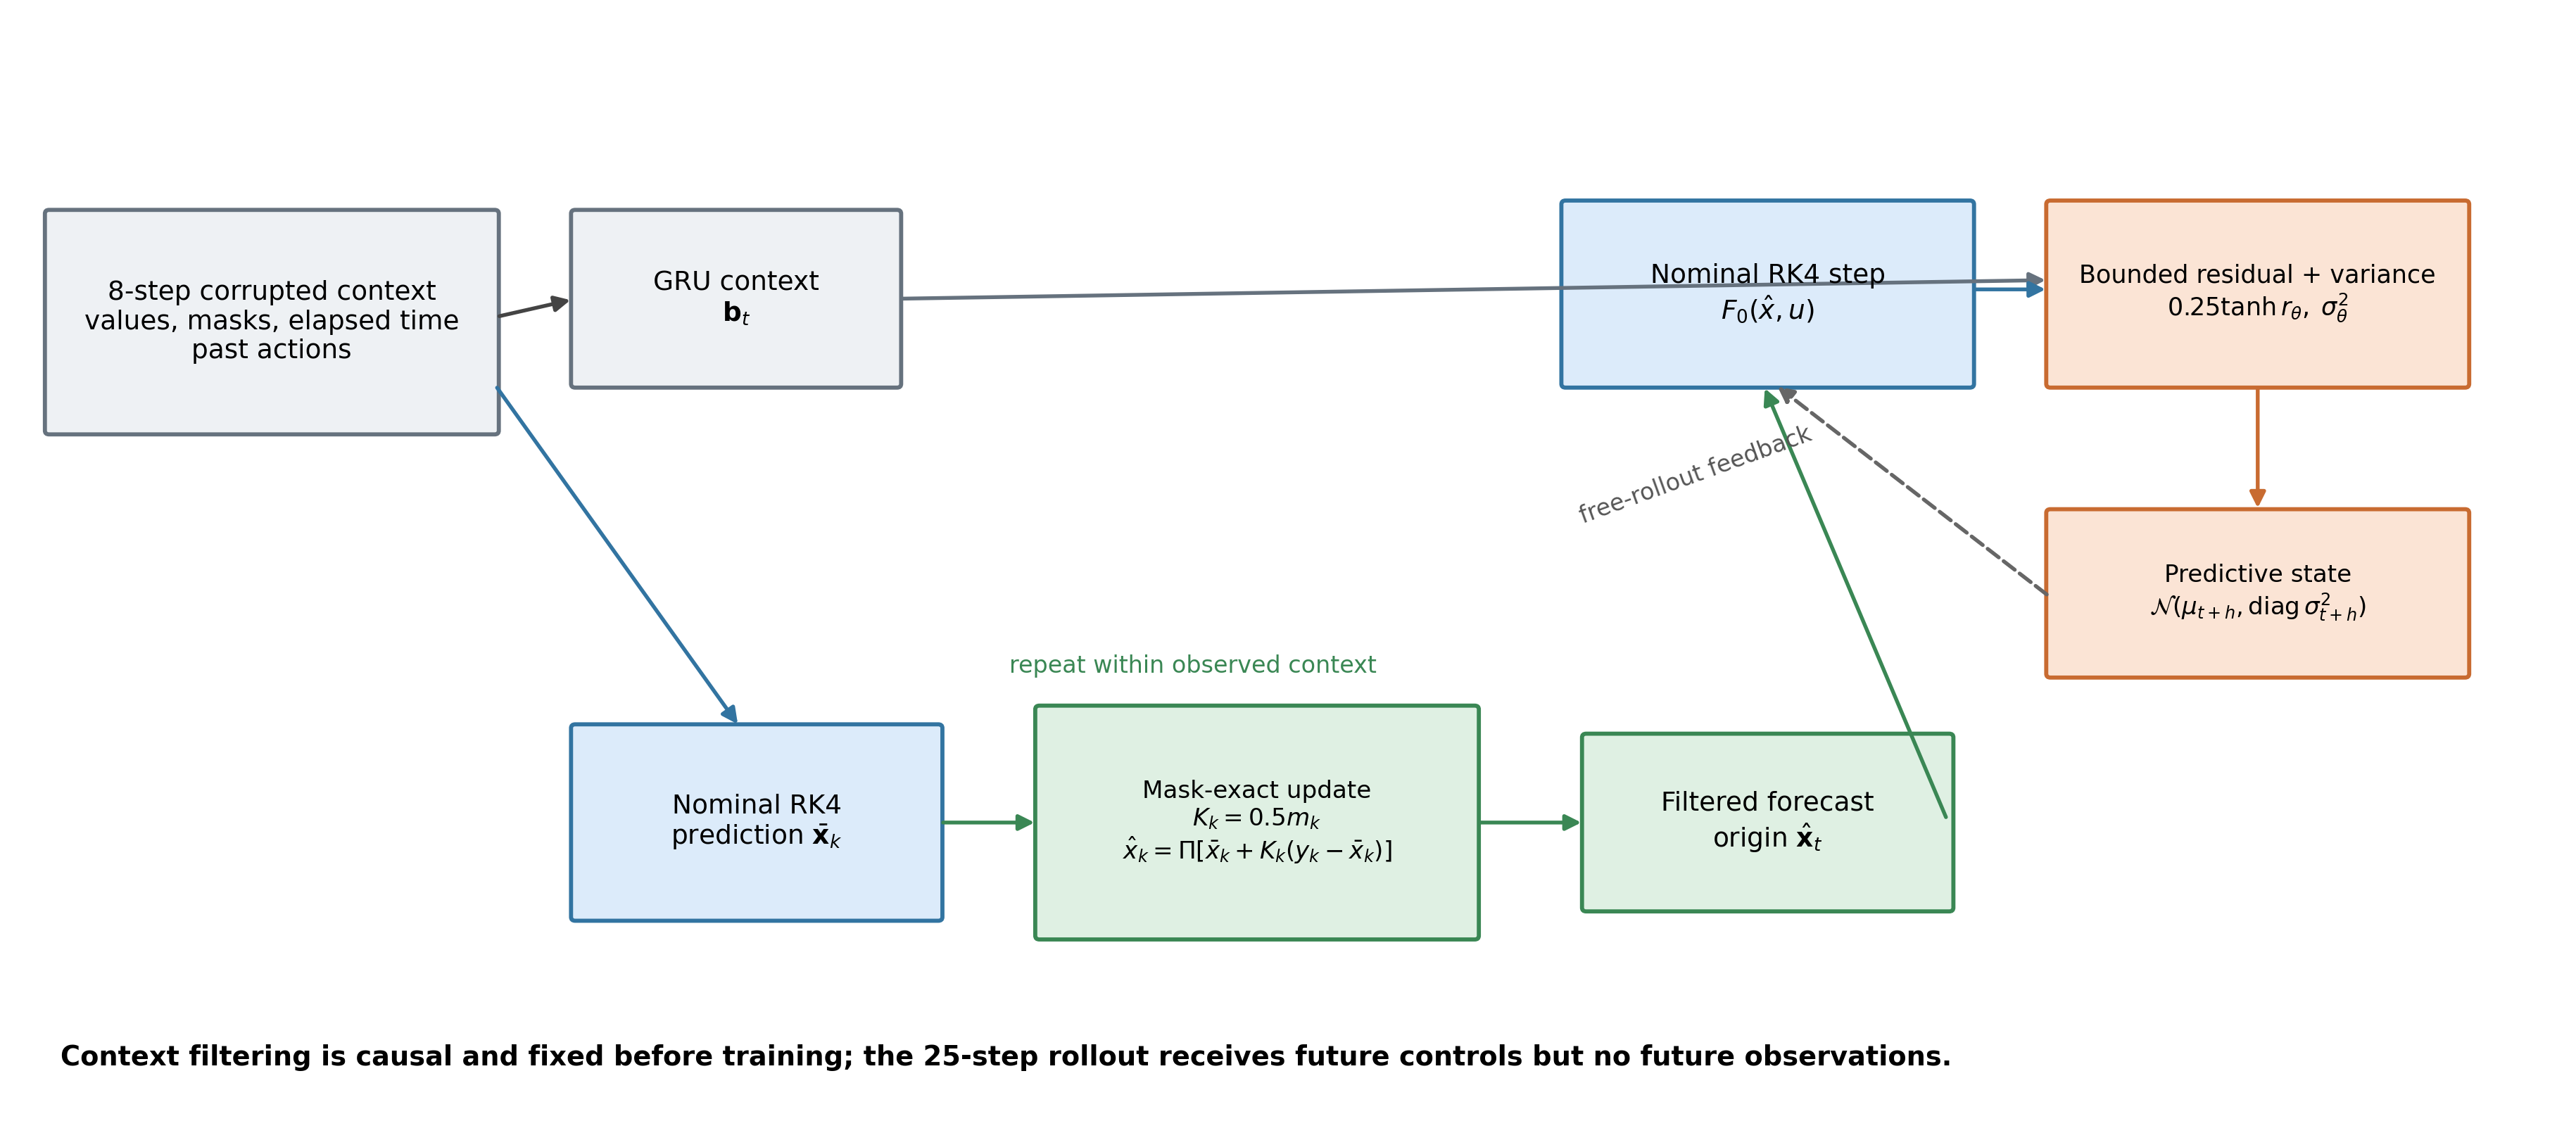
\includegraphics[width=0.96\textwidth]{figures/figure1_method.png}
\caption{Causal data flow of \method{}. A fixed complementary update is applied only inside the observed context. Missing channels receive exactly zero measurement gain. The filtered forecast origin then initializes a probabilistic nominal-physics plus neural-residual transition, which is rolled out freely for 25 steps using known future controls and no future observations.}
\label{fig:method}
\end{figure*}

\subsection{Forecasting problem}

Let $\vect{x}_t\in\mathbb{R}^{d_x}$ be a physical state and
$\vect{u}_t\in\mathbb{R}^{d_u}$ a recorded control. The observation available
to the model is
\begin{equation}
 \vect{y}_t=\vect{m}_t\odot(\vect{x}_t+\boldsymbol{\epsilon}_t),
\end{equation}
where $\vect{m}_t\in\{0,1\}^{d_x}$ is a channel-wise availability mask and
$\boldsymbol{\epsilon}_t$ is observation noise. Missing entries are filled
causally by the latest available value, producing $\tilde{\vect{y}}_t$; the
mask and elapsed time since observation $\boldsymbol{\delta}_t$ remain explicit
inputs, so an imputed value is never represented as a fresh measurement.

At forecast origin $t$, the model receives eight context states and their past
controls,
\begin{equation}
 \mathcal C_t=\{\tilde{\vect y}_{t-7:t},\vect m_{t-7:t},
 \boldsymbol\delta_{t-7:t},\vect u_{t-7:t-1}\},
\end{equation}
together with known future controls $\vect u_{t:t+H-1}$. It estimates a
diagonal predictive distribution for $\vect{x}_{t+1:t+H}$ under free rollout,
with $H=25$. Future states or observations are never fed back. All learned
operations use affine statistics estimated from the training split; the
nominal equations are evaluated in physical coordinates and then returned to
normalized coordinates.

\subsection{Mask-exact complementary context filter}

Let $F_0$ be one fourth-order Runge--Kutta step of a nominal controlled
differential equation. Starting from the first imputed context vector, the
filter alternates nominal prediction and measurement update. For context index
$k>t-7$,
\begin{align}
 \bar{\vect x}_{k} &= F_0(\hat{\vect x}_{k-1},\vect u_{k-1}),\\
 \vect K_k &= \alpha\vect m_k,\qquad \alpha=0.5,\\
 \hat{\vect x}_k &= \Pi\!\left[
 \bar{\vect x}_k+\vect K_k\odot
 (\tilde{\vect y}_k-\bar{\vect x}_k)\right].
 \label{eq:complementary-update}
\end{align}
Thus, before projection, an observed channel receives equal weight from the
nominal prediction and the current measurement, while a missing channel has
exactly zero measurement correction. The projection $\Pi$ is the identity
except for the sine--cosine pendulum representation, which is returned to the
unit circle after each update. That joint projection can alter either pendulum
channel even when its own measurement gain is zero, so the implementation does
not claim channel-wise equality to nominal propagation after projection. The
gain is fixed before training and has no access to validation or test outcomes.

In parallel, a GRU encodes
$[\tilde{\vect y}_k,\vect m_k,\log(1+\boldsymbol\delta_k),\vect u_{k-1}]$.
Its last hidden state supplies trajectory context to the forecast transition;
it does not alter the fixed measurement gain. The implementation retains the
same unused gain-head parameterization in every fixed-gain sensitivity model,
so comparisons at gains 0, 0.25, 0.5, 0.75, and 1 do not change nominal
capacity. We do not claim that complementary or Kalman-style filtering is new;
KalmanNet and modern data-assimilation work establish the broader prior art
\cite{revach2022_kalmannet,cheng2023_machine_learning_with_data_assimilation}.
The tested contribution is the use of a prespecified, mask-exact context update
as the forecast origin of a physics-residual probabilistic world model.

\subsection{Probabilistic physics-residual rollout}

The last filtered context state initializes a free rollout. At step $h$,
\begin{align}
 \boldsymbol\mu^{p}_{t+h} &= F_0(\hat{\vect x}_{t+h-1},\vect u_{t+h-1}),\\
 [\vect r_{t+h},\vect \ell_{t+h}] &=
 R_\theta([\hat{\vect x}_{t+h-1},\vect u_{t+h-1},\vect b_{t+h-1}]),\\
 \boldsymbol\mu_{t+h} &= \Pi\!\left[
 \boldsymbol\mu^{p}_{t+h}+0.25\tanh(\vect r_{t+h})\right],\\
 \boldsymbol\sigma^2_{t+h} &=
 \max\!\left\{\exp\!\left(\operatorname{clip}(\vect\ell_{t+h},-8,4)\right),
 10^{-6}\right\}.
 \label{eq:residual-rollout}
\end{align}
The fixed residual scale bounds a single normalized correction but does not
guarantee a bounded trajectory because errors can accumulate. The predicted
mean becomes the next state, and a GRUCell updates $\vect b$ from that mean and
the known control. No sampled state or future target enters the recurrence.

The training loss is the mean diagonal Gaussian negative log likelihood over
all $H$ steps and state channels,
\begin{equation}
 \mathcal L_{\mathrm{NLL}}=
 \frac{1}{2Hd_x}\sum_{h=1}^{H}\sum_{q=1}^{d_x}
 \left[\log(2\pi\sigma^2_{hq})+
 \frac{(x_{hq}-\mu_{hq})^2}{\sigma^2_{hq}}\right].
 \label{eq:nll}
\end{equation}
The one-step ablation applies the same loss only at $h=1$ but is still
evaluated by a 25-step free rollout.

\subsection{Causal execution and computational cost}

For each window, execution follows four deterministic stages. First, the GRU
encodes the imputed context together with masks, elapsed times, and past
controls. Second, Equation~\eqref{eq:complementary-update} advances the nominal
state through the same context and applies the mask-exact correction after each
available observation. Third, the final hidden state and filtered state jointly
initialize the residual recurrence. Fourth, Equation~\eqref{eq:residual-rollout}
is iterated for every known future control; predicted means, rather than samples
or targets, feed the next step. Training backpropagates the multi-step NLL
through this entire causal graph. Evaluation uses the identical graph with
gradients disabled, so teacher forcing is absent from both validation and test
rollouts.

Let $T_c$ denote context length, $H$ forecast horizon, $d_b$ recurrent width,
and $C_{F_0}$ the cost of one nominal RK4 step. Dense recurrent operations cost
$O((T_c+H)d_b^2)$ per trajectory, while nominal propagation costs
$O((T_c+H)C_{F_0})$. Diagonal mean and variance storage is $O(Hd_x)$; recurrent
working memory at inference is $O(d_b+d_x)$. Thus inference grows linearly in
context and horizon. The analysis does not claim asymptotic superiority over
the comparators: the fixed filter adds nominal context steps, and measured
latency is reported as an implementation property rather than a theoretical
speed advantage.

\subsection{Error decomposition and claim boundary}

For an observed scalar channel on which $\Pi$ is the identity, write the
nominal pre-update error as $e_p=\bar x-x$ and measurement error as
$\epsilon=y-x$. Before any non-identity projection, Equation
\eqref{eq:complementary-update} gives the exact post-update error
\begin{equation}
 e_f=(1-\alpha)e_p+\alpha\epsilon.
\end{equation}
If these errors are zero-mean and uncorrelated, then
\begin{equation}
 \mathbb E[e_f^2]=(1-\alpha)^2\mathbb E[e_p^2]
 +\alpha^2\mathbb E[\epsilon^2].
 \label{eq:filter-mse}
\end{equation}
Equal trust is therefore not universally optimal: it helps only when the two
error sources are sufficiently balanced, and a missing channel receives no
direct measurement-error term because its gain is zero. For the pendulum's
joint sine--cosine projection, an additional coupled projection error must be
accounted for, so Equation~\eqref{eq:filter-mse} is not asserted channel-wise
after projection. This conditional identity, rather than an optimal-filter
claim, motivates the fixed-gain sensitivity analysis.

If the rollout transition is locally $L$-Lipschitz and incurs local error
$\eta_h$, the standard recursion yields
\begin{equation}
 \|\hat{\vect x}_{t+H}-\vect x_{t+H}\|
 \le L^H\|\hat{\vect x}_t-\vect x_t\|
 +\sum_{h=0}^{H-1}L^{H-1-h}\eta_h.
\end{equation}
The context filter can reduce only the initial-error term; the residual model
must control subsequent local errors. Neither relation provides an
unconditional stability guarantee or supports claims about visual
representation learning, policy quality, or real-robot transfer.

\section{Experimental design}

\subsection{Controlled systems, corruption, and shift}

We evaluate five action-conditioned nonlinear systems. The damped oscillator
has state $(q,\dot q)$ and dynamics $m\ddot q+c\dot q+kq=u$; the Duffing
oscillator follows $\ddot q+c\dot q+\alpha q+\beta q^3=u$; and the controlled
Van der Pol system follows
$\ddot q=\mu(1-q^2)\dot q-q+g_u u$. The pendulum is represented by
$(\sin\theta,\cos\theta,\dot\theta)$, and the cart--pole by
$(x,\dot x,\theta,\dot\theta)$. Reference trajectories use fourth-order
Runge--Kutta integration with four internal substeps. Initial conditions,
bounded filtered stochastic controls, and physical parameters are generated
from recorded seeds. Shifted parameter intervals are prespecified and disjoint
from training intervals; unit tests verify that separation.

Each seed--system dataset contains 256 training, 64 validation, and 96 ID test
trajectories, plus 96 independently generated OOD test trajectories. A
trajectory has 72 states. Windows contain eight context states and 25 forecast
transitions; training and validation strides are eight and 16, respectively,
whereas evaluation uses one window per trajectory. Split identifiers encode
system, parameter regime, split, trajectory index, and generation seed. No
trajectory crosses splits.

The three deployment regimes are (i) clean ID context, (ii) ID context with
feature-wise Gaussian noise at 8\% of the mean training-state standard
deviation and a nominal 25\% independent missing-at-random probability, and
(iii) the same corruption with OOD physical parameters. Training context uses
3\% noise and a nominal 10\% missing probability. The first time point of every
generated trajectory is forced observed in every channel so causal last-value
imputation is defined; masks at all subsequent trajectory time points are
sampled independently. A later sliding window can therefore begin at an
unobserved, causally imputed context value. Masks and channel-wise elapsed times
are retained. ID-clean and ID-corrupt evaluations reuse the same underlying 96
trajectories, permitting repeated-measurement resampling. OOD identifiers are
required to be disjoint from ID identifiers.

\subsection{Comparators, sensitivities, and development firewall}

The five broad comparators cover recurrent, normalized, transformer, and
physics-guided transition families. \textbf{RSSM-style} is a compact recurrent
stochastic-style transition. \textbf{SimNorm-style} applies grouped simplex
normalization to its recurrent representation, adapting a representation
principle used by scalable continuous-control world models
\cite{hansen2023_td_mpc2_scalable_robust_world}. \textbf{Transformer-style} uses a
two-layer causal context transformer followed by recurrent free rollout
\cite{micheli2022_transformers_are_sample_efficient_world}. \textbf{PGNN-style}
adds a deterministic neural correction to a nominal physics step
\cite{robinson2022_physics_guided_neural_networks_for}. \textbf{PG-DMM-style} is a
probabilistic physics-residual transition inspired by physics-guided Deep
Markov modeling \cite{liu2022_physics_guided_deep_markov_models}. These are
protocol-matched transition implementations, not reproductions of published
end-to-end agents or their reported returns.

The proposed \textbf{\method} uses gain 0.5. Four fixed-gain sensitivities use
$\alpha\in\{0,0.25,0.75,1\}$, and \textbf{CFR-one-step} changes only the
training horizon. All six CFR variants have hidden width 72 and identical
parameterization; even the inactive fixed-gain head is retained. Comparator
widths are 80 for RSSM-style and SimNorm-style, 48 for Transformer-style, and
84 for PGNN-style and PG-DMM-style.

Candidate selection was separated from confirmation. A first development
model, reliability-gated RGP-WM, failed its corrected primary hypothesis after
an audit replaced a trajectory-local NRMSE denominator by a training-only
scale. A structurally distinct learned-gain PFR-WM then improved over retrained
the PGNN-style comparator on development seed 11, but exceeded its prespecified gain-0.5 matched
ablation by only 0.223\%, below the frozen 2\% mechanism threshold. Learned
gain was therefore rejected and is absent from every confirmatory seed. The
gain-0.5 comparator from that failed mechanism test became the versioned
CFR-WM candidate before confirmation. Original development outputs, corrected
re-evaluations, and failure decisions remain archived; none is pooled with the
confirmatory analysis.

\subsection{Optimization and endpoint definitions}

All models use AdamW, batch size 128, gradient clipping at norm 5, at most 60
epochs, and early stopping after ten epochs without a validation-NLL
improvement of $10^{-5}$. The pre-confirmation tuning archive contains the same
six-trial validation budget for every baseline--system pair. Each baseline uses
its own frozen winner. CFR-WM and all CFR sensitivities inherit the frozen PGNN-style
winner for the same system, preventing an additional candidate-specific search.
No confirmatory result can alter a hyperparameter.

The primary endpoint is NRMSE through horizon 25. Per-feature RMSE is divided
by that feature's standard deviation estimated from the training split only,
then averaged over features. Because stored targets and predictions are already
in those normalized coordinates, the evaluation divisor is one. This avoids
estimating a denominator from the test trajectory and remains defined at
horizon one. Secondary accuracy endpoints are cumulative NRMSE at horizons 1,
5, and 10 and MAE through horizon 25. Probabilistic endpoints are diagonal
Gaussian NLL, empirical 90\% coverage, mean 90\% interval width, and mean
absolute central-interval calibration error over nominal levels 0.1--0.9. A
trajectory is catastrophic when any feature-step absolute error exceeds three
training-set standard deviations.

\subsection{Frozen confirmatory inference}

The confirmation grid contains 11 methods, eight untouched seeds
$(41,53,67,79,83,97,109,113)$, five systems, and three regimes: 440 training
runs, 1,320 aggregate cells, and 126,720 paired trajectory rows. One
deterministic dataset fingerprint is shared by all methods within each
seed--system group, and all 40 such fingerprints must be distinct. The eight
seed-level training/data realizations are the top-level independent clusters;
trajectories are nested observations. Systems and regimes are treated as a
fixed benchmark, so inference does not imply sampling from a population of all
physical systems.

For a seed $s$, let $B_s$ and $C_s$ be the PGNN-style and CFR-WM NRMSE-25 means after
equal weighting of all 15 system--regime cells. The primary estimand is
\begin{equation}
 \Delta_{\mathrm{rel}}=\frac{1}{8}\sum_{s=1}^{8}
 100\frac{B_s-C_s}{B_s}.
 \label{eq:primary-estimand}
\end{equation}
A 5,000-replicate bootstrap resamples seeds globally with replacement. Within
each selected seed and system it resamples paired trajectory identifiers;
ID-clean and ID-corrupt reuse the same sampled identifier vector, while the
disjoint OOD set is resampled independently. Every system--regime cell is
retained, and $B_s$, $C_s$, and their ratio are recomputed in each replicate.
The interval is the two-sided percentile 95\% interval.

H1 states that \method{} improves on the preselected PGNN-style comparator by at least 5\%.
Support requires finite metrics, a lower relative-improvement interval endpoint
of at least 5\%, and a one-sided exact sign-flip $p<0.05$ for the seed effects
after subtracting the 5\% margin. All $2^8$ sign configurations are enumerated
under a prespecified symmetry assumption. Confirmation success is determined
by H1 alone.

H2 is tested only if H1 succeeds. It requires at least 5\% improvement when
pooling ID-corrupt and OOD-corrupt fixed cells, and clean-regime
noninferiority with signed relative-improvement margin $-5\%$. Both components
must meet their respective bootstrap bound and one-sided margin test, with all
metrics finite. The five broad CFR-versus-comparator contrasts form one Holm
family; the five CFR sensitivity/ablation contrasts form another. With eight
clusters, the minimum two-sided exact raw and five-test Holm-adjusted values are
$2/2^8=0.0078125$ and 0.0390625. The 15 system--regime contrasts report paired
effects and unadjusted bootstrap intervals only; they are explicitly
descriptive and carry no cell-level significance claim.

\subsection{Fail-closed reproducibility controls}

The machine-readable contract was frozen before the first confirmatory dataset.
It pins method and seed grids, data counts, optimization, estimands, margins,
multiplicity families, output location, and SHA-256 fingerprints for training
code, analysis code, and the tuning archive. The dedicated runner accepts no
overrides. Before data generation it checks all contract fields and hashes;
partial resume is allowed only for an exact provenance-bound subset with paired
JSON and checkpoint artifacts. The generic experiment CLI rejects every frozen
seed and the reserved output directory before loading tuning or generating
data. The analyzer independently revalidates the contract, current code,
payload configurations, 40 distinct dataset fingerprints, exact row grid,
paired trajectory identifiers, and finite values. Intermediate confirmatory
metrics are not inspected.

The first invocation of the frozen analyzer stopped before any bootstrap,
decision, or result file because its generic loader omitted the already stored
top-level \texttt{parameter\_count} field required only by the descriptive
model-size summary. Before inspecting any performance output, we froze a
versioned analysis amendment that performs one validated many-to-one join on
method, seed, and system, then calls the unchanged confirmatory and statistical
functions. It also rechecks all 440 JSON/checkpoint pairs and refuses to
overwrite an analysis directory. The original contract, failed zero-output
logs, amendment, and their hashes are retained; no outcome, estimand, margin,
random seed, bootstrap count, or decision rule changed.

Execution uses Python 3.11.15 and PyTorch 2.11.0+cu130 on an NVIDIA RTX 5070
Laptop GPU with 8,151 MiB reported memory and an AMD Ryzen 9 9955HX processor.
The sequential runner stops at 80\% of an eight-hour budget, writes each
condition atomically, and never synthesizes missing performance values.

\section{Results}

\subsection{Integrity checks and aggregate accuracy}

The confirmatory analyzer accepted the complete grid of \ConfirmatoryRuns{}
trained models and \ConfirmatoryTrajectories{} trajectory-level rows. All
prespecified metrics were finite (\AllMetricsFinite), and the 40 seed--system
groups produced \UniqueDataHashes{} distinct data fingerprints while sharing
one fingerprint across methods within each group. These checks establish grid
completeness and pairing; they are not performance evidence.

Table~\ref{tab:main-results} reports the seed-balanced mean and standard
deviation for horizons 1, 10, and 25. Across all 11 methods, \BestMethod{}
had the lowest aggregate NRMSE-25 (\BestNRMSE). CFR-WM's mean was
\CFRNRMSE{}, compared with \PGNNNRMSE{} for the preselected PGNN-style comparator.
This ordering is descriptive: confirmatory support depends on paired
seed-level effects and frozen practical margins, not on the lowest pooled mean
alone.
The confirmatory estimand does not follow solely from these pooled means: it
averages eight within-seed relative effects after giving every fixed
system--regime cell equal weight.

\begin{table*}[t]
\centering
\caption{Confirmatory accuracy over the fixed five-system, three-regime
benchmark. Entries are means $\pm$ SD across eight seed-level, cell-balanced
aggregates. Bold marks the lowest aggregate NRMSE-25; it does not by itself
denote confirmatory support. Parameter counts are means over the five
system-specific input dimensions; all methods received the same six-trial
validation search budget.}
\label{tab:main-results}
\resizebox{\textwidth}{!}{\begin{tabular}{lrrrr}
\toprule
Method & Mean parameters & NRMSE-1 & NRMSE-10 & NRMSE-25 \\
\midrule
CFR-WM & 57694 & 0.039 $\pm$ 0.001 & 0.057 $\pm$ 0.002 & \textbf{0.100 $\pm$ 0.004} \\
CFR-gain-0.25 & 57694 & 0.037 $\pm$ 0.001 & 0.059 $\pm$ 0.002 & 0.103 $\pm$ 0.004 \\
CFR-gain-0.75 & 57694 & 0.047 $\pm$ 0.001 & 0.065 $\pm$ 0.002 & 0.107 $\pm$ 0.005 \\
PGNN-style & 61275 & 0.060 $\pm$ 0.001 & 0.070 $\pm$ 0.002 & 0.110 $\pm$ 0.003 \\
CFR-gain-1 & 57694 & 0.059 $\pm$ 0.001 & 0.073 $\pm$ 0.002 & 0.114 $\pm$ 0.004 \\
PG-DMM-style & 61493 & 0.063 $\pm$ 0.001 & 0.075 $\pm$ 0.002 & 0.114 $\pm$ 0.003 \\
RSSM-style & 62485 & 0.073 $\pm$ 0.002 & 0.090 $\pm$ 0.005 & 0.123 $\pm$ 0.006 \\
Transformer-style & 59708 & 0.074 $\pm$ 0.002 & 0.094 $\pm$ 0.004 & 0.132 $\pm$ 0.009 \\
SimNorm-style & 62485 & 0.074 $\pm$ 0.002 & 0.098 $\pm$ 0.006 & 0.138 $\pm$ 0.013 \\
CFR-gain-0 & 57694 & 0.081 $\pm$ 0.003 & 0.100 $\pm$ 0.003 & 0.144 $\pm$ 0.005 \\
CFR-one-step & 57694 & 0.040 $\pm$ 0.001 & 0.136 $\pm$ 0.050 & 0.278 $\pm$ 0.104 \\
\bottomrule
\end{tabular}
}
\end{table*}

\begin{quote}
\small\textbf{Frozen primary estimand.} For each seed, PGNN-style and CFR-WM
NRMSE-25 are first averaged with equal weight over the 15 prespecified
system--regime cells; their relative improvement is then computed. The
confirmatory point estimate is the arithmetic mean of those eight seed-level
relative improvements, not the ratio of the two pooled means in
Table~\ref{tab:main-results}.
\end{quote}

\subsection{Primary and gated robustness hypotheses}

Against PGNN-style, the seed-mean relative NRMSE-25 improvement was
\PrimaryImprovement\% (95\% paired fixed-cell bootstrap CI
[\PrimaryRelativeCILow\%, \PrimaryRelativeCIHigh\%]). In absolute units,
CFR-WM minus PGNN-style was \PrimaryDifference{} (95\% CI [\PrimaryCILow,
\PrimaryCIHigh]). The exact one-sided sign-flip test against the same 5\%
practical margin gave $p=\PrimaryPValue$. Under the frozen conjunction of a
5\% interval lower bound, $p<0.05$, and finite metrics, H1 was
\PrimaryDecision. This decision is not changed by rankings against other
comparators or by favorable individual cells.

For the H2 components, the combined corrupt-ID and corrupt-OOD regimes had a
relative effect of \CorruptImprovement\% (95\% CI
[\CorruptRelativeCILow\%, \CorruptRelativeCIHigh\%], one-sided 5\%-margin
$p=\CorruptPValue$). ID-clean had an effect of \CleanImprovement\% (95\% CI
[\CleanRelativeCILow\%, \CleanRelativeCIHigh\%], one-sided signed
$-5\%$-margin $p=\CleanPValue$). Because H2 is hierarchically gated by H1 and
requires both component rules, the robustness hypothesis was
\RobustnessDecision.

Table~\ref{tab:seed-effects} exposes the eight independent cluster effects
rather than only their mean. Every seed exceeded the 5\% practical threshold,
although the exact test still treats the seed effects as the inferential units.

\begin{table}[t]
\centering
\caption{Seed-level primary effects after equal weighting of the 15 frozen
benchmark cells. Positive values favor CFR-WM.}
\label{tab:seed-effects}
\begin{tabular}{rr}
\toprule
Seed & CFR-WM improvement over PGNN-style, \% \\
\midrule
41 & +5.29 \\
53 & +12.76 \\
67 & +12.01 \\
79 & +10.49 \\
83 & +9.69 \\
97 & +6.66 \\
109 & +9.32 \\
113 & +5.56 \\
\bottomrule
\end{tabular}

\end{table}

\begin{figure*}[t]
\centering
\includegraphics[width=0.96\textwidth]{figures/confirmatory_overview.png}
\caption{Locked confirmatory summary. (A) Aggregate transition accuracy for the
six main methods. (B) Paired CFR-WM effects against PGNN-style by regime; positive
values favor CFR-WM. (C) Prespecified fixed-gain sensitivity. (D) Paired
fixed-cell intervals against each broad comparator. Error bars in A--C are
seed-level SD; D uses the nested 95\% bootstrap interval.}
\label{fig:confirmatory-overview}
\end{figure*}

\subsection{Comparator and sensitivity evidence}

Table~\ref{tab:comparator-contrasts} reports every prespecified broad
comparison. Positive relative effects favor CFR-WM. The confidence intervals
retain all fixed cells, whereas the exact two-sided seed sign-flip values are
Holm-adjusted as one five-test family. These comparisons contextualize H1 but
do not replace its preselected PGNN-style contrast or its 5\% margin.

The PGNN-style row repeats the primary point estimate but uses the frozen
comparator-family bootstrap seed (20260808), whereas H1 uses its prespecified
primary seed (20260805). The estimand and 5,000-replicate resampling scheme are
otherwise identical; the separately sampled interval endpoints differ by at
most 0.01 percentage point after rounding, and only the primary interval enters
the H1 decision.

\begin{table*}[t]
\centering
\caption{CFR-WM relative NRMSE-25 effects against broad comparators. Exact
$p$ values test a zero seed-level difference; Holm adjustment is confined to
this prespecified family of five.}
\label{tab:comparator-contrasts}
\begin{tabular}{lrrr}
\toprule
Reference & Relative effect [95\% CI], \% & Exact $p$ & Holm $p$ \\
\midrule
RSSM-style & +19.08 [+17.16, +20.98] & 0.0078 & 0.0391 \\
SimNorm-style & +27.34 [+24.00, +30.62] & 0.0078 & 0.0391 \\
Transformer-style & +24.09 [+21.65, +26.64] & 0.0078 & 0.0391 \\
PGNN-style & +8.97 [+6.89, +10.96] & 0.0078 & 0.0391 \\
PG-DMM-style & +12.44 [+10.51, +14.39] & 0.0078 & 0.0391 \\
\bottomrule
\end{tabular}

\end{table*}

The lowest aggregate NRMSE-25 among gains $0$, $0.25$, $0.5$, $0.75$, and $1$
occurred at gain \BestGain. Relative to the one-step-trained variant, CFR-WM's
effect was \OneStepImprovement\% (95\% CI [\OneStepRelativeCILow\%,
\OneStepRelativeCIHigh\%], Holm $p=\OneStepHolmP$). Table
\ref{tab:sensitivity-contrasts} gives the complete second five-test family;
therefore the gain sweep is reported even when it does not favor the proposed
value.

\begin{table*}[t]
\centering
\caption{CFR-WM relative NRMSE-25 effects against gain and training-horizon
sensitivities. Positive values favor the proposed gain-0.5 multi-step model.}
\label{tab:sensitivity-contrasts}
\begin{tabular}{lrrr}
\toprule
Reference & Relative effect [95\% CI], \% & Exact $p$ & Holm $p$ \\
\midrule
Gain 0 & +30.89 [+28.95, +32.67] & 0.0078 & 0.0391 \\
Gain 0.25 & +2.97 [+0.88, +5.27] & 0.0312 & 0.0391 \\
Gain 0.75 & +6.97 [+4.77, +9.42] & 0.0078 & 0.0391 \\
Gain 1 & +12.13 [+10.31, +13.92] & 0.0078 & 0.0391 \\
One-step training & +59.38 [+48.88, +68.88] & 0.0078 & 0.0391 \\
\bottomrule
\end{tabular}

\end{table*}

Secondary probabilistic metrics are shown in Table~\ref{tab:secondary}. They
are diagnostics rather than alternate confirmation endpoints: lower Gaussian
NLL, calibration error, or catastrophic-rollout rate cannot rescue a failed
H1, and diagonal-Gaussian calibration does not imply a correct joint forecast
distribution.

\begin{table*}[t]
\centering
\caption{Secondary aggregate diagnostics for the six broad methods. Rates and
scores are seed-balanced over all fixed cells and are not separately tested.}
\label{tab:secondary}
\resizebox{\textwidth}{!}{\begin{tabular}{lrrrr}
\toprule
Method & Parameters & Gaussian NLL & Calibration error & Catastrophic rate \\
\midrule
RSSM-style & 62485 & -0.183 & 0.214 & 0.01\% \\
SimNorm-style & 62485 & -0.246 & 0.206 & 0.01\% \\
Transformer-style & 59708 & -0.279 & 0.202 & 0.01\% \\
PGNN-style & 61275 & -0.385 & 0.248 & 0.00\% \\
PG-DMM-style & 61493 & 0.029 & 0.245 & 0.00\% \\
CFR-WM & 57694 & 0.013 & 0.228 & 0.00\% \\
\bottomrule
\end{tabular}
}
\end{table*}

\subsection{Fixed-cell heterogeneity}

Figure~\ref{fig:cell-heterogeneity} retains all 15 system--regime effects. By
the frozen descriptive guard, CFR-WM was more than 10\% worse than PGNN-style in
\CellsWorseTen{} cells. All three were ID-clean: cart--pole
(\CartpoleCleanChange\% relative change), controlled Van der Pol
(\VanDerPolCleanChange\%), and Duffing (\DuffingCleanChange\%). Conversely,
\IDCorruptFavoredCount{} of \IDCorruptCellCount{} ID-corrupt cells favored
CFR-WM, with descriptive changes from \IDCorruptLeastChange\% to
\IDCorruptMostChange\%. This pattern explains why an aggregate H1 success coexists with
failure of clean-regime noninferiority. No cell-level $p$ value is reported:
with eight seed clusters, those contrasts were not assigned confirmatory
multiplicity claims.
The exact estimates and unadjusted bootstrap intervals are archived in the
appendix table and machine-readable CSV.

\begin{figure}[t]
\centering
\includegraphics[width=\linewidth]{figures/cell_difference_heatmap.png}
\caption{Descriptive CFR-WM change relative to PGNN-style in each fixed benchmark
cell. Negative values mean lower NRMSE-25 for CFR-WM.}
\label{fig:cell-heterogeneity}
\end{figure}

\section{Discussion}

The frozen analysis \PrimaryInterpretation. This statement is deliberately
stronger than asking whether CFR-WM's point estimate is favorable: H1 required
the lower bootstrap endpoint to clear a 5\% practical margin and the exact
seed-level test to reject that same margin. The distinction matters with eight
top-level realizations, for which apparently stable trajectory-level averages
can coexist with substantial training-seed uncertainty. The result therefore
answers a narrow question about equal-trust context correction on the fixed
benchmark; it is neither a universal ranking of world-model architectures nor
a post hoc selection of the most favorable comparator.

The regime decomposition gives the proposed mechanism a more specific stress test. The
corrupt/shifted estimate was \CorruptImprovement\%, whereas the clean estimate
was \CleanImprovement\%; after hierarchical gating, the full analysis
\RobustnessInterpretation. Context corruption and parameter shift stress
different terms in the error recursion. Noise and missingness weaken the
measurement term in Equation~\eqref{eq:filter-mse}, while parameter shift biases
the nominal pre-update error and the subsequent nominal rollout. A gain of 0.5
cannot adapt between these cases. Consequently, similar aggregate effects can
mask different cell patterns. The three cells with more than 10\% degradation
were all clean, led by cart--pole, while every ID-corrupt cell improved
descriptively. This pattern is consistent with noise suppression within the
bundled corrupt regimes, but the design cannot separate Gaussian noise from
missingness or parameter shift; equal trust can also over-correct already
accurate clean context. This is why the regime effects and all 15 cells are
retained without promoting them to independent confirmatory or causal claims.

The gain sweep further prevents the fixed value from being interpreted as an
optimal filter. The descriptively lowest aggregate NRMSE among the five frozen
gains occurred at \BestGain. This result locates equal trust within a continuum
from pure nominal context propagation (gain 0) to direct measurement
replacement (gain 1). It does not estimate a Bayes-optimal gain, because the
noise, nominal-model error, and missingness processes vary by channel and
trajectory. A learned gain was considered during development, but its advantage
over the matched fixed-gain model missed a prespecified mechanism threshold;
excluding it from confirmation avoids relabeling residual-model capacity as
filter adaptation.

Multi-step training addresses a different part of the recursion. CFR-WM's
relative effect against the one-step-trained variant was
\OneStepImprovement\% (95\% CI [\OneStepRelativeCILow\%,
\OneStepRelativeCIHigh\%]). The context filter changes the initial-error term,
whereas multi-step likelihood exposes the residual transition to its own
forecast distribution and targets accumulated local errors. Their roles are
therefore complementary in the mathematical sense of the bound, even if the
Holm-adjusted sensitivity contrast does not support a population-level
component claim.

Relative to recent world-model and physics-guided work, the value of CFR-WM is
auditability rather than architectural scale. It uses a transparent
measurement rule, explicit missing-channel semantics, known-control free
rollout, and a fixed practical-effect gate. This design trades adaptive
expressivity for a mechanism that can be falsified with approximately
parameter-matched gains.
The archived failure of two earlier candidates is part of that evidence: it
shows that physics, uncertainty, or a learned gate cannot be treated as useful
merely because each is plausible in isolation. Future extensions should adopt
the same separation when adding visual encoders, structured occlusion,
ensembles or conformal calibration, and closed-loop planning
\cite{portela2025_conformal_prediction_for_uncertainty_quantification,brunke2022_safe_learning_in_robotics_from}.

Most importantly, the study distinguishes mathematical, simulated, and
deployment evidence. The filter identity is conditional; the benchmark
establishes measured predictive effects under explicit perturbations; neither
establishes causal mechanism, policy benefit, or hardware safety. Maintaining
those boundaries is necessary for a compact physical-world-model result to be
scientifically useful rather than rhetorically broader than its data.

\section{Limitations}

The evidential scope is intentionally narrower than the general world-model
problem. First, all trajectories come from five analytically specified,
low-dimensional controlled systems. This gives exact split, corruption, and
parameter-shift provenance, but it does not reproduce the visual ambiguity,
contacts, unmodeled objects, sensor synchronization failures, or nonstationary
actuation encountered by embodied agents. The state is directly observed
before synthetic corruption, future controls are supplied, and no policy is
trained. Prediction quality here therefore cannot be converted into a claim
about control return, planning safety, or real-robot transfer.

Second, every model receives the correct differential-equation family with
imperfect parameters. Structural misspecification, hidden state variables, and
informative sensor dropout may change the balance between nominal propagation
and measurement correction. The gain 0.5 is deliberately fixed rather than
estimated from uncertainty; the gain sweep measures sensitivity on this
benchmark but does not establish filter optimality. The Gaussian diagonal
forecast likewise cannot represent multimodality or full cross-state
covariance, and the bounded one-step residual does not guarantee stable
multi-step trajectories.

The two corrupt evaluation regimes bundle Gaussian observation noise and
missingness, and the OOD-corrupt regime additionally bundles parameter shift.
There are no noise-only, missingness-only, or clean-OOD factorial cells.
Accordingly, regime differences cannot identify which perturbation caused an
effect or establish the complementary update as its causal mechanism.

Third, inference has only eight independent seed-level training/data
realizations. The exact sign-flip test is attainable for the prespecified
five-comparison families, but it has coarse resolution and assumes symmetry of
seed effects. Trajectory resampling improves precision for the fixed benchmark
without creating additional independent training replicates. System--regime
contrasts are consequently descriptive, and all generalization claims remain
limited to the frozen five-system grid. Larger preregistered seed studies,
structurally wrong physics, state-dependent missingness, visual encoders, and
hardware-in-the-loop evaluation are necessary before deployment claims would
be justified.

\section{Conclusion}

We introduced CFR-WM, a compact world model that combines a prespecified,
mask-exact complementary context update with a probabilistic
physics-residual transition. The design isolates two sources of long-horizon
error: uncertainty in the state at the forecast origin and error accumulated by
the free-rollout transition. A conditional error identity explains when the
fixed update can help, while gain and training-horizon sensitivities test its
limits without claiming universal filtering optimality.

The confirmatory study trained \ConfirmatoryRuns{} models across five
controlled nonlinear systems, three deployment regimes, eight independent
seed-level realizations, five broad comparators, and five sensitivities. Against
the preselected PGNN-style baseline, the seed-balanced relative NRMSE-25 effect was
\PrimaryImprovement\% (95\% CI [\PrimaryRelativeCILow\%,
\PrimaryRelativeCIHigh\%]); accordingly, H1 was \PrimaryDecision, but the
prespecified H2 robustness claim was \RobustnessDecision{} because clean
noninferiority failed. Specifically, the corrupt/shifted component improved while clean-regime
noninferiority failed, exposing the cost of a nonadaptive equal-trust update.
These decisions follow the frozen 5\% practical margin and exact seed-level
tests, not a favorable pooled mean or selected system.

The work contributes both a technical composition and an evidential pattern:
simple physics-aware corrections should be evaluated against matched
sensitivities, and unsuccessful development mechanisms should remain visible
rather than being absorbed into confirmation. The present evidence is limited
to state-transition prediction with known controls on a synthetic-mechanistic
benchmark. The next defensible steps are preregistered evaluation with
structurally misspecified physics and informative missingness, followed by
visual state estimation and hardware-in-the-loop closed-loop control. Those
extensions require new safety, calibration, and policy endpoints; they cannot
be inferred from NRMSE alone.

\backmatter

\section*{Declarations}

\textbf{Funding} [To be completed by the authors before submission.]

\textbf{Competing interests} The authors declare no competing interests.

\textbf{Ethics approval and consent to participate} Not applicable. The study uses analytically simulated controlled dynamics and no human participants, animals, or personal data.

\textbf{Consent for publication} Not applicable.

\textbf{Data and code availability} All trajectories are generated from the controlled differential equations supplied with the source package. The package contains generation seeds, split identifiers, checkpoints, trajectory-level metrics, the frozen confirmatory contract, and scripts for every table and figure. A public archival repository and persistent identifier must be added before submission.

\textbf{Author contributions} [To be completed by the authors before submission.]

\textbf{Generative-AI assistance} Generative-AI tools assisted drafting and software development. The authors retain responsibility for the final text and verified the equations, source metadata, code outputs, statistical results, and claims against the archived artifacts. This statement must be reconciled with the publisher policy in force on the submission date.

\begin{appendices}
% Keep Hyperref destinations unique when the Springer class resets appendix counters.
\renewcommand{\theHtable}{appendix.\arabic{table}}
\renewcommand{\theHfigure}{appendix.\arabic{figure}}
\renewcommand{\theHequation}{appendix.\arabic{equation}}
\section{Benchmark specification}

Table~\ref{tab:systems} records the simulator time step and nominal
parameterization; Table~\ref{tab:parameter-ranges} gives every sampled training
and OOD interval. All OOD intervals are non-overlapping on every named shifted
parameter. The ranges are benchmark definitions, not a claim that they exhaust
physically meaningful behavior.

\begin{table*}[ht]
\centering
\caption{Controlled-system definitions. $u$ is scalar in every system.}
\label{tab:systems}
\resizebox{\textwidth}{!}{%
\begin{tabular}{llll}
\toprule
System & State & $\Delta t$ & Nominal parameters \\
\midrule
Damped oscillator & $(q,\dot q)$ & 0.050 & $m=1.0,\; k=1.6,\; c=0.18$ \\
Forced Duffing & $(q,\dot q)$ & 0.040 & $\alpha=-1.0,\;\beta=1.0,\;c=0.25$ \\
Controlled Van der Pol & $(q,\dot q)$ & 0.035 & $\mu=1.2,\;g_u=1.0$ \\
Torque pendulum & $(\sin\theta,\cos\theta,\dot\theta)$ & 0.040 & $g=9.81,\;l=1.0,\;m=1.0,\;c=0.12$ \\
Cart--pole & $(x,\dot x,\theta,\dot\theta)$ & 0.025 & $g=9.81,\;m_c=1.0,\;m_p=0.1,\;l/2=0.5,\;c=0.04$ \\
\bottomrule
\end{tabular}}
\end{table*}

\begin{table*}[ht]
\centering
\scriptsize
\caption{Complete independently sampled physical-parameter intervals. Symbols
follow Table~\ref{tab:systems}; $g_u$ is the Van der Pol control gain.}
\label{tab:parameter-ranges}
\resizebox{\textwidth}{!}{%
\begin{tabular}{lll}
\toprule
System & Training interval & OOD interval \\
\midrule
Damped oscillator & $m\in[0.90,1.10],\ k\in[1.40,1.80],\ c\in[0.14,0.22]$ & $m\in[1.25,1.45],\ k\in[2.05,2.35],\ c\in[0.26,0.34]$ \\
Forced Duffing & $\alpha\in[-1.10,-0.90],\ \beta\in[0.90,1.10],\ c\in[0.20,0.30]$ & $\alpha\in[-0.75,-0.60],\ \beta\in[1.25,1.45],\ c\in[0.34,0.44]$ \\
Controlled Van der Pol & $\mu\in[1.00,1.40],\ g_u\in[0.90,1.10]$ & $\mu\in[1.65,1.95],\ g_u\in[1.25,1.45]$ \\
Torque pendulum & $g\in[9.65,9.95],\ l\in[0.90,1.10],\ m\in[0.90,1.10],\ c\in[0.08,0.16]$ & $g\in[10.25,10.55],\ l\in[1.25,1.45],\ m\in[1.25,1.45],\ c\in[0.20,0.28]$ \\
Cart--pole & $g\in[9.65,9.95],\ m_c\in[0.90,1.10],\ m_p\in[0.085,0.115],\ l/2\in[0.45,0.55],\ c\in[0.02,0.06]$ & $g\in[10.25,10.55],\ m_c\in[1.25,1.45],\ m_p\in[0.135,0.160],\ l/2\in[0.65,0.78],\ c\in[0.075,0.105]$ \\
\bottomrule
\end{tabular}}
\end{table*}

The action generator is a bounded first-order filtered process. At step $t$, a Gaussian innovation with scale $0.55$ times the system action limit is combined with the previous action using coefficients 0.18 and 0.82, then clipped. Limits are 1.5, 1.8, 1.2, 2.2, and 8.0 for the systems in Table~\ref{tab:systems}. This produces persistent excitation without using the simulated state as feedback. It is part of the input distribution, not a learned behavior policy.

Train/validation/test separation occurs before window construction. A root NumPy \texttt{SeedSequence} spawns distinct split generators, which in turn spawn one generator per trajectory. The OOD test has a separate root seed. Observation corruption uses another recorded seed after state generation. Consequently, changing an observation-noise level does not change the underlying clean ID trajectory, and all methods see exactly the same corruption draw within a condition.

\section{Development firewall and confirmatory grid}

Two earlier candidates were screened before the present confirmation. The first, RGP-WM, was rejected after correcting an inappropriate trajectory-local normalization in the development analysis. The second, a learned-gain PFR-WM, was rejected by its frozen kill rule because its NRMSE-25 improvement over the prespecified gain-0.5 sensitivity was only 0.223\%, below the required 2\%. Neither candidate appears in the confirmatory grid. The fixed gain of 0.5 used by CFR-WM was selected from that prespecified development sensitivity before any confirmatory seed was generated. These development outcomes motivate the design but provide no evidence for the confirmatory claims.

The immutable grid comprises 11 methods, eight seeds (41, 53, 67, 79, 83, 97, 109, and 113), five systems, and three test regimes. It therefore contains 440 fitted models, 1,320 aggregate evaluation cells, and 126,720 trajectory-level rows. Each seed--system dataset contains 256 training, 64 validation, and 96 test trajectories of 72 time steps. Models receive eight context steps and predict 25 steps open loop. Training observations use noise equal to 3\% of the fixed training-state scale and a nominal 10\% independent missing probability; the corrupt regimes use 8\% observation noise and a nominal 25\% probability. The first time point of each generated trajectory is forced observed in every channel, with independent masks sampled at all subsequent trajectory times; a later sliding-window context can begin with an imputed value. ID-clean and ID-corrupt evaluations share trajectory identifiers; the OOD trajectory set is disjoint.

The five broad comparators are compact, protocol-matched RSSM-style,
SimNorm-style, Transformer-style, PGNN-style, and PG-DMM-style transitions.
They are not exact reproductions of the cited end-to-end systems. Five
prespecified CFR sensitivities test gains $0$, $0.25$, $0.75$, and $1$, plus a
one-step-trained gain-0.5 model. CFR-WM retains the unused learned-gain-head
parameters so that fixed-gain comparisons do not obtain a parameter-count
advantage by removing that head.

All methods ingest normalized context values, masks, log-one-plus elapsed times,
and actions. Except for the Transformer-style encoder, context is encoded by a
GRU; open-loop recurrent updates use a GRUCell. Every MLP has two hidden linear
layers with SiLU activation. Table~\ref{tab:architectures} lists the remaining
architecture-specific choices.

\begin{table*}[ht]
\centering
\scriptsize
\caption{Exact compact transition architectures used in the confirmatory grid.
The bounded correction is $0.25\tanh(\cdot)$ and all forecast covariances are
diagonal.}
\label{tab:architectures}
\resizebox{\textwidth}{!}{%
\begin{tabular}{llll}
\toprule
Method & Width & Context representation & Forecast transition and variance \\
\midrule
RSSM-style & 80 & GRU; sigmoid feature scaling & data-only MLP mean/log-variance; GRUCell rollout \\
SimNorm-style & 80 & GRU; eight-group simplex projection & data-only MLP mean/log-variance; GRUCell rollout \\
Transformer-style & 48 & two causal layers, four heads, FF width 96, GELU, dropout 0 & data-only MLP mean/log-variance; GRUCell rollout \\
PGNN-style & 84 & GRU & nominal one-substep RK4 plus deterministic residual MLP; learned constant log-variance \\
PG-DMM-style & 84 & GRU & nominal one-substep RK4 plus residual mean/log-variance MLP \\
CFR-WM and gain sensitivities & 72 & GRU states plus mask-exact fixed-gain context update & nominal one-substep RK4 plus residual mean/log-variance MLP \\
\bottomrule
\end{tabular}}
\end{table*}

For CFR-WM, observed context channels use gain 0.5 and missing channels use
gain 0 exactly. The learned gain head remains instantiated but is inactive.
The four gain sensitivities change only the observed-channel gain; the
one-step sensitivity changes only the likelihood horizon.

\section{Frozen hyperparameter search}

The same six learning-rate/weight-decay trials were run on development seed 11
for every system--baseline pair (Table~\ref{tab:tuning-grid}). The stored
reliability-loss weight is shown because it is part of the generic training
configuration, but it is inactive for all confirmatory methods in this paper.
Each baseline uses the validation-NLL winner in
Table~\ref{tab:tuning-winners}; CFR-WM and all CFR sensitivities inherit the
PGNN-style winner for the same system.

\begin{table}[ht]
\centering
\caption{Six-trial frozen optimization grid.}
\label{tab:tuning-grid}
\begin{tabular}{rrrr}
\toprule
Trial & Learning rate & Weight decay & Stored $\lambda_{\mathrm{rel}}$ \\
\midrule
0 & $3\times10^{-4}$ & $10^{-6}$ & 0.1 \\
1 & $6\times10^{-4}$ & $10^{-5}$ & 0.2 \\
2 & $10^{-3}$ & $10^{-5}$ & 0.2 \\
3 & $1.5\times10^{-3}$ & $10^{-4}$ & 0.3 \\
4 & $2\times10^{-3}$ & $10^{-5}$ & 0.4 \\
5 & $3\times10^{-3}$ & $10^{-4}$ & 0.2 \\
\bottomrule
\end{tabular}
\end{table}

\begin{table*}[ht]
\centering
\caption{Frozen winning trial index by system and protocol-matched baseline.}
\label{tab:tuning-winners}
\resizebox{\textwidth}{!}{%
\begin{tabular}{lrrrrr}
\toprule
System & RSSM-style & SimNorm-style & Transformer-style & PGNN-style & PG-DMM-style \\
\midrule
Damped oscillator & 3 & 2 & 4 & 5 & 1 \\
Forced Duffing & 5 & 4 & 5 & 5 & 5 \\
Controlled Van der Pol & 5 & 5 & 5 & 5 & 0 \\
Torque pendulum & 5 & 5 & 5 & 5 & 4 \\
Cart--pole & 5 & 5 & 5 & 5 & 5 \\
\bottomrule
\end{tabular}
}
\end{table*}

\section{Confirmatory estimands and decisions}

H1 is the sole confirmation gate. It asks whether CFR-WM improves fixed-training-scale NRMSE-25 over the preselected PGNN-style comparator by at least 5\%. Within each seed, PGNN-style and CFR-WM are averaged with equal weight over all 15 fixed system--regime cells; the primary point estimate is the arithmetic mean of the eight seed-specific relative improvements. H1 requires finite metrics, a 95\% bootstrap lower endpoint of at least 5\%, and a one-sided exact sign-flip $p<0.05$ for the 5\% margin.

H2 is a hierarchically gated robustness claim. Conditional on H1, the combined corrupt and parameter-shifted regimes must satisfy the same 5\% improvement rule, while ID-clean performance must be noninferior under a signed relative margin of $-5\%$. Both components require their corresponding bootstrap lower endpoint to meet or exceed the margin and a one-sided exact sign-flip $p<0.05$. If H1 fails, H2 is not supported irrespective of its component estimates.

The bootstrap uses 5,000 replicates. Each replicate resamples the eight seed clusters globally with replacement and then resamples paired trajectory identifiers within every retained seed--system block. A single sampled identifier vector is reused for ID-clean and ID-corrupt repeated measurements, whereas the disjoint OOD identifiers are sampled separately. All five systems and three regimes remain in every replicate, and baseline, candidate, and their relative ratio are recomputed within the replicate. Exact tests enumerate all $2^8$ seed-level sign flips and therefore rely on a seed-effect symmetry assumption. The five broad-comparator contrasts and the five sensitivity contrasts form separate Holm-adjusted families. The 15 system--regime contrasts are descriptive and carry no cell-level significance claim.

\section{Integrity and scope boundaries}

The frozen contract records the method list, seeds, data design, training configuration, success rules, and SHA-256 hashes of the training, evaluation, analysis, and tuning artifacts. The dedicated runner rejects command-line overrides and resumes only provenance-matched JSON/checkpoint pairs. The generic development runner rejects every frozen seed and the reserved confirmatory output directory. Analysis aborts unless the exact grid, finite metrics, trajectory pairing, disjoint OOD identifiers, 40 distinct seed--system data hashes, and stored provenance all validate.

The first frozen-analysis invocation failed before inferential resampling and wrote no result directory because the generic loader had not copied the existing top-level \texttt{parameter\_count} metadata into the aggregate frame used for descriptive model-size reporting. The archived amendment was frozen before performance inspection. It adds only that field by a method--seed--system many-to-one join, verifies all 440 JSON/checkpoint pairs and the completed-run manifest, and then invokes the unchanged frozen inference functions. The failed log, original analysis hash, amendment code hash, and amendment-contract hash are included in the reproduction package. No trajectory metric, hypothesis, threshold, resampling seed, replicate count, multiplicity family, or decision changed.

The top-level independent units are the eight stochastic training/data realizations; trajectories are nested observations and are not treated as independent experimental replicates. Statistical claims therefore concern this prespecified finite benchmark and variation across the frozen seed realizations. They do not establish universal superiority across physical systems, hardware platforms, sensing stacks, control policies, or real-world deployment conditions.

\section{Complete descriptive cell contrasts}

Table~\ref{tab:all-cell-contrasts} reports every prespecified CFR-WM--PGNN-style
system--regime contrast. Absolute intervals come from the paired nested
bootstrap. Relative changes use PGNN-style as the denominator, with negative values
favoring CFR-WM. These fixed-cell estimates are descriptive: no cell-level
significance decision or multiplicity-adjusted $p$ value was prespecified.

\begin{table*}[ht]
\centering
\small
\caption{All 15 descriptive CFR-WM versus PGNN-style NRMSE-25 contrasts.}
\label{tab:all-cell-contrasts}
\resizebox{\textwidth}{!}{\begin{tabular}{llrr}
\toprule
System & Regime & CFR--PGNN-style [95\% CI] & Relative change, \% \\
\midrule
Cartpole & ID clean & +0.0163 [+0.0103, +0.0225] & +47.33 \\
Cartpole & ID corrupt & -0.0207 [-0.0281, -0.0136] & -13.33 \\
Cartpole & OOD + corrupt & -0.0111 [-0.0194, -0.0027] & -5.66 \\
Controlled Van Der Pol & ID clean & +0.0059 [-0.0022, +0.0149] & +19.36 \\
Controlled Van Der Pol & ID corrupt & -0.0318 [-0.0381, -0.0250] & -32.39 \\
Controlled Van Der Pol & OOD + corrupt & -0.0083 [-0.0148, -0.0016] & -4.74 \\
Damped Oscillator & ID clean & -0.0011 [-0.0041, +0.0019] & -2.41 \\
Damped Oscillator & ID corrupt & -0.0291 [-0.0341, -0.0244] & -32.12 \\
Damped Oscillator & OOD + corrupt & -0.0257 [-0.0295, -0.0223] & -27.86 \\
Forced Duffing & ID clean & +0.0094 [+0.0028, +0.0168] & +24.37 \\
Forced Duffing & ID corrupt & -0.0295 [-0.0342, -0.0249] & -30.24 \\
Forced Duffing & OOD + corrupt & +0.0094 [+0.0011, +0.0174] & +3.90 \\
Torque Pendulum & ID clean & -0.0046 [-0.0082, -0.0005] & -8.59 \\
Torque Pendulum & ID corrupt & -0.0378 [-0.0436, -0.0316] & -34.80 \\
Torque Pendulum & OOD + corrupt & +0.0110 [+0.0055, +0.0165] & +5.94 \\
\bottomrule
\end{tabular}
}
\end{table*}
\end{appendices}

\bibliography{../references}
\end{document}
